\documentclass{article}
\usepackage[utf8]{inputenc}
\usepackage{pdfpages}
\begin{document}
\begin{figure}
\centering

\includegraphics[scale=0.25]{ulco.png}
\label{fig:ucp}\\%
\end{figure}


\title{SOLITAIRE MORPION IN Q-LEARNING}
\maketitle


\begin{center}
\centering
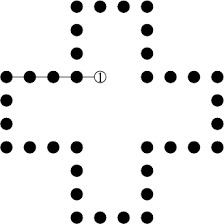
\includegraphics[scale=0.7]{logosm.png}
\label{fig:ucp}\\%
\end{center}

\begin{center}
\author{Author :}\\%
Anis MEZRAG 
\end{center}
\begin{center}
\author{Tutor}\\%
Denis ROBILLIARD
\end{center}
 \newpage
    \tableofcontents
\newpage
\part{Thanks}
\paragraph{}
\setlength{\parindent}{2cm}
First of all, it seems appropriate to express our thanks to all those who helped us in the realisation of this project, in particular our supervisor Mr Denis ROBILLIARD, from whom we were able to benefit from a great deal of support.
\newpage
\section{Introduction}
\subsection{Principle of the game}
\paragraph{}
\setlength{\parindent}{2cm}
The Morpion Solitaire is a puzzle that can be solved alone. Inspired by Morpion. It is played with paper and pencil. It consists in drawing a maximum of lines of 4 or 5 elements starting from a figure in the shape of a Greek cross.

\subsection{Presentation of the project}
\paragraph{}
\setlength{\parindent}{2cm}
The project consists in realizing a python algorithm that can detect all the possible lines to be played in each game. The first objective is to make it play randomly and then to connect it to an artificial neural network. The goal is to run the algorithm to optimize its score thanks to reinforcement learning.

\subsection{Rules of the game}
\paragraph{}
\setlength{\parindent}{2cm}
Starting configuration with a Greek cross formed by 36 points.\paragraph{}
\setlength{\parindent}{2cm}
Example of a solitary Morpion game, 5 points in a row, after 3 moves.
The game is played on a grid (supposedly of unlimited size). The starting configuration consists of a set of stitches (or small crosses) already drawn on this grid; the most common configurations place these stitches in the shape of a Greek cross whose side has 3 stitches (24 in total) or 4 stitches (36 in total).
\paragraph{}
\setlength{\parindent}{2cm}
With each move, the player places a new point on the grid so as to form a row of four or five adjacent points horizontally, vertically or diagonally (the number of points in a row is decided before the game, according to the initial configuration, and remains fixed throughout the game) and then connects this row with a pencil stroke.
\paragraph{}
\setlength{\parindent}{2cm}
Depending on the chosen rule, a line-up may or may not be placed as an extension of a previous line-up. If the player has this possibility, the two lines of play can only have one point in common.
\paragraph{}
\setlength{\parindent}{2cm}
The object of the game is to place as many points as possible before reaching a situation where no new points can be placed.
~\cite{solitaire} 
\subsection{Comparative study with existing solutions}
\subsubsection{Highest score by Chris Rosin}
\paragraph{}
\setlength{\parindent}{2cm}
 The last record, on August 12, 2011, with 178 strokes! And again from
 Chris Rosin, a step up from his previous record announced
 only three months earlier, using an improved version of
 the method described in its article IJCAI. New record
 immediately announced by the Pour La Science website, also by
 Tangent N143 of Nov-Dec 2011. Chris lives in San Diego,
 California since 1992, and is a co-founder of Parity.
 Computing where he is Chief Algorithmist. His personal page is
Translated with www.DeepL.com/Translator (free version)
 www.chrisrosin.com
 ~\cite{score} 
\begin{center}
\centering
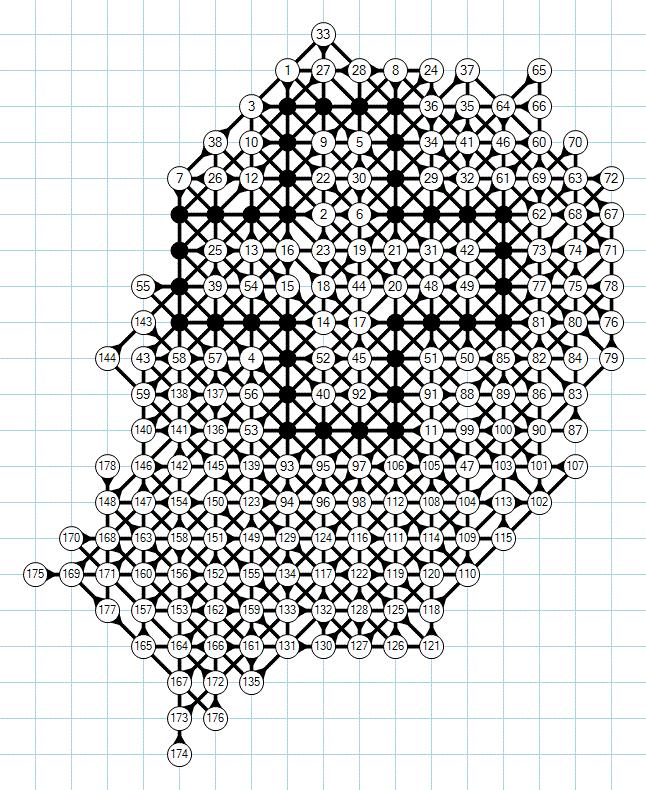
\includegraphics[scale=0.4]{Capture d’écran 2020-06-12 à 13.52.04.png}
\label{fig:ucp}\\%
\end{center}
\subsubsection{Analyzing symmetrical grids, Michael Quist}
\paragraph{}
\setlength{\parindent}{2cm}
Analyzing by computer the symmetrical grids, Michael Quist, USA, found this excellent and very beautiful grid of 136 moves, so only 10 moves less than the above record!
He thinks this should be the maximum score of all symmetrical 5Ts grids (symmetrical with respect to the center like this one, but also diagonally symmetrical, horizontally symmetrical, 90 rotation, ...).~\cite{chinois} 
\begin{figure}
\centering
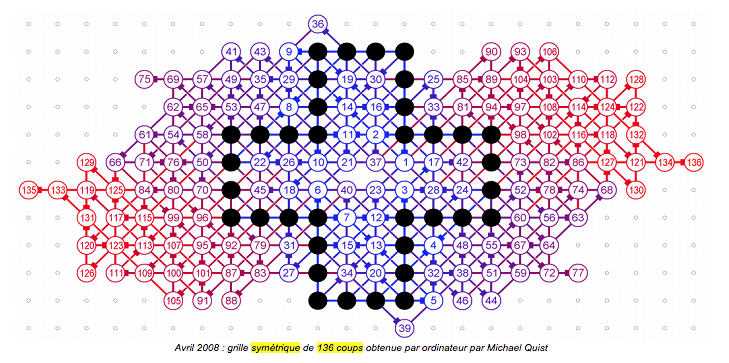
\includegraphics[scale=0.4]{Capture d’écran 2020-06-12 à 13.42.12.png}
\end{figure}
\subsubsection{Study by Jean-Jacques Sibilla}
\paragraph{}
\setlength{\parindent}{2cm}
Jean-Jacques Sibilla, IPGP (http://www.ipgp.fr/~sibilla), is carrying out an
interesting research: since 2007, her computer has generated two
billion grids (status as of October 2013), where the moves are played
randomly. Its main results:
\newline
- Extremely difficult to obtain grids of more than 100 strokes, its
best grid with 102 hits-two peaks at 21 and 64 hits
\newline
- Impossible to get less than 20 shots, as mentioned in the
worst possible grids
~\cite{score} 
\begin{center}
\centering
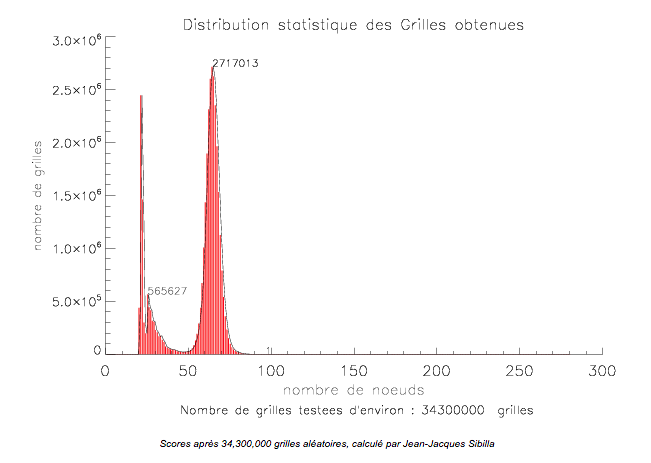
\includegraphics[scale=0.3]{Capture d’écran 2020-06-12 à 13.42.41.png}
\label{fig:ucp}\\%
\end{center}

\subsection{Interest of the game}
\paragraph{}
\setlength{\parindent}{2cm}
The problem of finding long sequences of solitary tic-tac-toe can be approached in several ways. In our work, two of these approaches are of particular interest: reinforcement learning methods, and random methods based on complete searches of playable lines and playing randomly one after the other.Some of the algorithms we present search for sequences from the initial position. Some of the algorithms we present search for sequences from the initial position, while others are used to perform complete cell searches. One usefulness of these algorithms, however, is that they can be used to improve on good sequences that have already been found. ~\cite{these} 
\newpage
\part{Design and development environment}
\section{Software environment}
\subsection{Design and development tools}
\subsubsection{PyCharm}
\paragraph{}
\setlength{\parindent}{2cm}
PyCharm is an integrated development environment used for
programming in Python. It allows code analysis and contains a
graphics debugger. It also allows the management of tests
integration of version management software, the integration of unitary.~\cite{pycharm} 
\paragraph{}
\setlength{\parindent}{2cm}
The advantages of this software are numerous, in particular the free of charge and its use on several platforms such as Unix, Windows or Mac Os. All Python libraries are available in one click. It is a powerful and complete tool, particularly adapted for the computer implementation of artificial intelligence methods.

\subsubsection{Anaconda}
\paragraph{}
\setlength{\parindent}{2cm}
Anaconda is a free and open source distribution of the languages of
Python and R programming applied to application development
dedicated to data science and machine learning,
which aims to simplify package management and deployment.
Package versions are managed by the
conda5 packages. The Anaconda distribution is used by more than 6
million users and includes more than 250 popular packages in
data science suitable for Windows, Linux and MacOS.
~\cite{anaconda} 
\subsection{Technological choices}
\subsubsection{Python}
\paragraph{}
\setlength{\parindent}{2cm}
For the programming language of the algorithm we started with Python because it is an interpreted, multi-paradigm and multi-platform programming language. It promotes structured, functional and object-oriented imperative programming.~\cite{python}  
It is also appreciated because it provides a language where the syntax, clearly separated from low-level mechanisms, allows an easy introduction to the basic concepts of programming.

\subsubsection{LaTeX}
\paragraph{}
\setlength{\parindent}{2cm}
For the drafting of the documents related to this project, we started on Latex. It allows us to write documents whose layout is done automatically, conforming as much as possible to typographical standards. A distinguishing feature of latex is its mathematical mode, which allows complex formulas to be composed. Latex is particularly used in the technical and scientific fields for the production of medium-sized documents (such as articles) or important documents (theses or books, for example). Nevertheless, it can be used to generate a wide variety of document types.
~\cite{latex} 
\section{Conception}
\subsection{Beginning of the project}
\subsubsection{The first steps}
\paragraph{}
\setlength{\parindent}{2cm}
When we started the project we started by studying the game Snake, which was it, already connected to the neural network and perfectly functional.  We also tried to understand, in a general way, what is Q learning or learning by reinforcement.
\paragraph{}
\setlength{\parindent}{2cm}
It helped us a lot in understanding the game.  We understood that we had to detect all the states that change as the game progresses.  We had a meeting with our tutor who helped us to better understand the problems of each project and then to choose the one that suited us best. We chose the solitaire game Morpion.

\subsubsection{Progress in versions}
\paragraph{}
\setlength{\parindent}{2cm}
The first version of the project was to make an engine calculating all the playable cells and how they are played the disadvantage of this version was that the code had more than 1700 lines with console display the compilation was very slow. a more elaborate version was then considered by removing the console display by replacing it with a much graphical interface that provides a better display a faster compilation speed. 

\paragraph{}
\setlength{\parindent}{2cm}
 After several exchanges with our tutor, another version has
This was achieved this time by transforming the 1700 lines into less than 200, thanks to the shortcut offered by the python language.

\newpage
\subsection{Artificial neural network design}
\subsubsection{Description of the Q-Learning concept}
\paragraph{}
\setlength{\parindent}{2cm}
In artificial intelligence, more precisely in automatic learning, Q-learning is a learning technique by reinforcement. This technique does not require any initial model of the environment. The letter 'Q' designates the function that measures the quality of an action executed in a given state of the system.
One of the strong points of Q-learning is that it allows you to compare the likely rewards of taking accessible actions without any initial knowledge of the environment. In other words, although the system is modelled by a Markovian (finite) decision process, the learning agent does not know it and the Q-learning algorithm does not use it. 
~\cite{learning} 
\newline
\begin{figure}[!h]
\centering
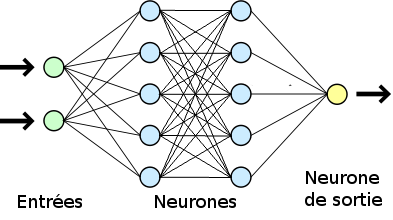
\includegraphics[scale=0.5]{neurones.png}
\\% 
\caption{Example of an artificial neural network}
\end{figure}

\subsubsection{Implementation of Q-Learning in our project}
\paragraph{}
\setlength{\parindent}{2cm}
Taking inspiration from the snake game, we understood that the first objective was to find repetitive elements that best describe the state of the game. We started with different approaches to define these elements. We tried to work on the list of playable lines, ordering their playability. We looked for the line that would create the most playable lines and gave an indication of its position in relation to the centre, but without any concrete learning result because the game was dependent and deterministic.
\paragraph{}
\setlength{\parindent}{2cm}
Then we changed our approach. We divided the square one game into three, and o giving in the states an indication by polar coordinates, in which of the three games there is the most playable line, but in vain. 
\paragraph{}
\setlength{\parindent}{2cm}
Finally, the last approach that led to concrete results was to decrease the determinism of the game, by creating a player with a distance of freedom (Its implementation and functioning are explained in Development 4.4). We are constantly changing states, we came across a formula where the game starts with random moves giving poor results and after 50 games, the player starts to see the dangés and make the right moves to play more and more lines.
\newpage
\part{Development and functionalities}
\section{Development}
\subsection{Algorithm}
\paragraph{}
\setlength{\parindent}{2cm}
The main algorithm of the game quotes to scan all the cells of the game looking for playable lines. all playable lines can be detected from the first cell and this searches for 24 cells aligned click play magnet on the direction align. counts this condition is verified, the line is added to the directory of playable lines with all the cells of the line and the direction of the line.

\subsection{Game Engine}
\subsubsection{Class Cellule}
\paragraph{}
\setlength{\parindent}{2cm}
 The Cell class represents a cell in the game. It contains seven attributes, five of which are Booleans. The first four are to say whether the square has already been played vertically, horizontally, diagonally left or diagonally right. The seventh ball that is "clicked" tells us whether the square and clicked or not.   As for the last two, they indicate the coordinates (x, y) of the square or a cell. 
\begin{figure}[!h]
\centering
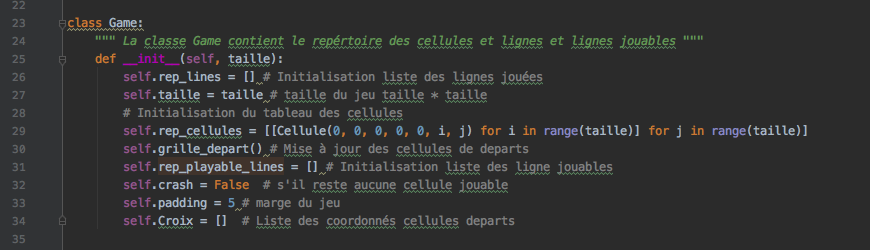
\includegraphics[scale=0.4]{cellule.png}
\\% 
\caption{Code of the class Cellule}
\end{figure}

 \paragraph{}
\setlength{\parindent}{2cm}
This class contains a method get attribute by index and this closed method to return the value of an attribute of the class cell with its index.
\subsubsection{La classe Game}
\paragraph{}
\setlength{\parindent}{2cm}
  The class range has as attribute "size", this one represents the number of square or cells on one side of the square of the game. In our case we used a size which is equal to 30 which allows us to create therefore nine hundred cells.
 \paragraph{}
\setlength{\parindent}{2cm}
\begin{figure}[!h]
\centering
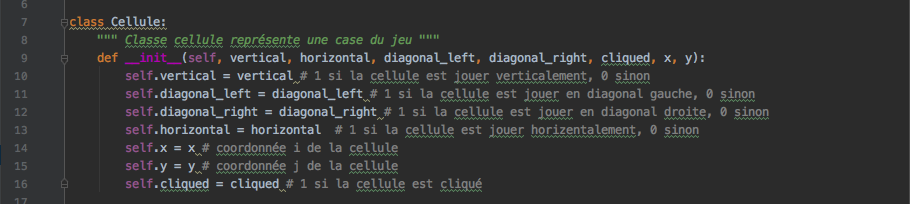
\includegraphics[scale=0.4]{game.png}
\\% 
\caption{Code of the class Game}
\end{figure}
the method "starting grid" allows to initialize the first cells of the game (the Greek cross), by putting them as clicked so that the differentiators of the other squares.
\subsubsection{The method of detecting playable lines}
\paragraph{}
\setlength{\parindent}{2cm}
Algorithm It starts by initializing the list of the directory of playable lines. Then we created a list of four vectors that summarize the index change in the four main directions, i.e. vertical, horizontal, left diagonal and right diagonal. Next, we made two nested loops that run through all the cells of the game making conditions to find at least four in five (4/5) cells that are aligned, clicked and not played in the direction of the cell. Finally, they are added to the list of playable rows, which will then be used to check whether a cell is playable or not.  
 \begin{figure}[!h]
\centering
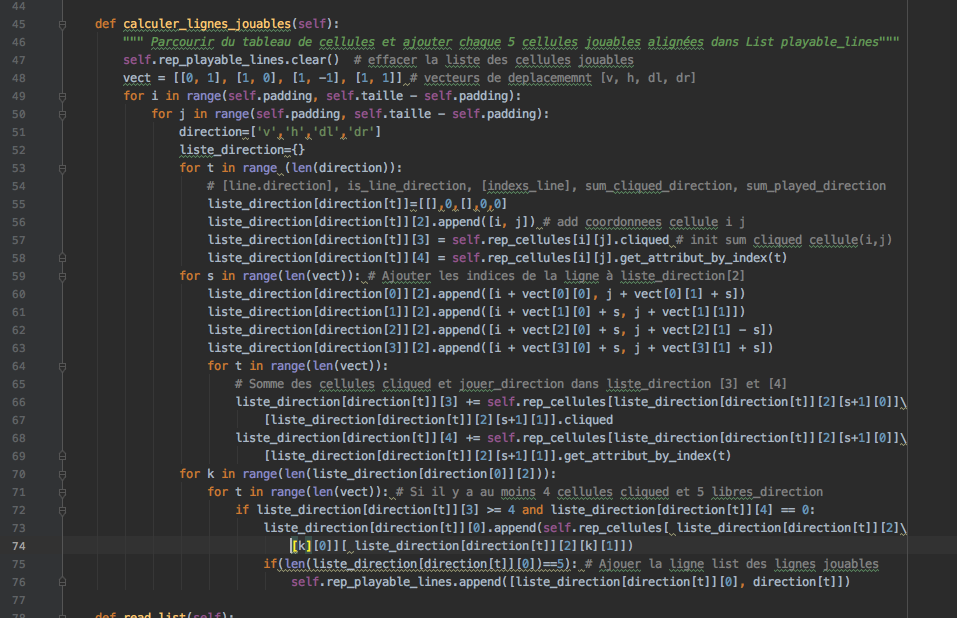
\includegraphics[scale=0.36]{main.png}
\\% 
\caption{Code of the method that calculates playable lines}
\end{figure}
\subsubsection{The method for playing a line}
\paragraph{}
\setlength{\parindent}{2cm}
'Jouer-ligne' is a method that takes a line as a parameter. First, it checks if it is not empty. The line attribute is a list that contains two components. The first contains the five cells of the row. The second, on the other hand, contains the direction in which it is playable.

\subsubsection{The method 'Main'}
 The 'main' method is the method is the entry point of the algorithm. It is where control of the program begins and ends. The first lines but this method was used to initialize the parameters of the game i.e. the size of the game, as well as the initialization of the GUI. 
\begin{figure}[!h]
\centering
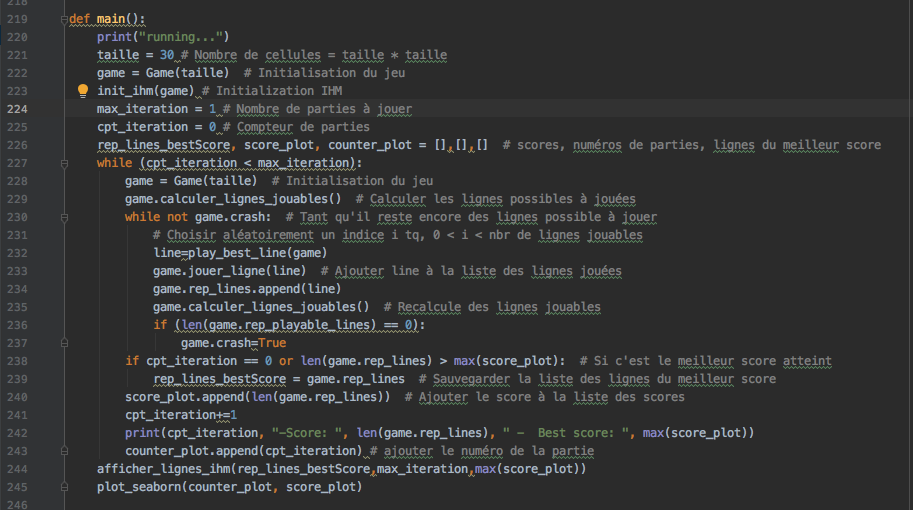
\includegraphics[scale=0.4]{search.png}
\\% 
\caption{Code of the method Main}
\end{figure}
 \paragraph{}
\setlength{\parindent}{2cm}
 You also initialize the maximum number of games and the game counter, the list of high score lines, high scores and games. However, as long as the game counter has not reached the maximum, the game class is initialized. Then the playable lines are calculated. Afterwards, we choose randomly among the playable lines that will serve as an indication for the agent in the states. 
\subsection{Graphical user interface}
\paragraph{}
\setlength{\parindent}{2cm}
The graphical user interface contains a total of five main methods. These will allow you to visualize all the elements of the game, including the lines created at the end and two counters, one for the number of games played and the other to indicate the best score. The interface also allows to display the evolution of the game with the score of each game played and this on two different parts with the display of the lines.
\subsubsection{Method 'constructeur'}
\paragraph{}
\setlength{\parindent}{2cm}
This method makes it possible to draw all the squares of the game and to put in bold the starting cells that are clicked. 
\subsubsection{Mehtod 'init-ihm'}
\paragraph{}
\setlength{\parindent}{2cm}
'init-ihm' takes as scale attribute, allows to draw the square of the game as well as the two small counters, the number of games is the maximum score reached.
\subsubsection{Méthode 'afficher-ligne-ihm'}
\paragraph{}
\setlength{\parindent}{2cm}
 This method is called at the end of the game to draw all the lines created when the game has reached its best score. It takes as an attribute a list of the lines created, the number of games played and the best score.
\subsubsection{Method 'plot-seaborn'}
\paragraph{}
\setlength{\parindent}{2cm}
plot-seaborn is a method that will allow us, at the end of the game, to represent each score according to the number of games played. Thus draw a line according to the method of the least squares to visualize the evolution at each game. 
\newline
\begin{figure}[!h]
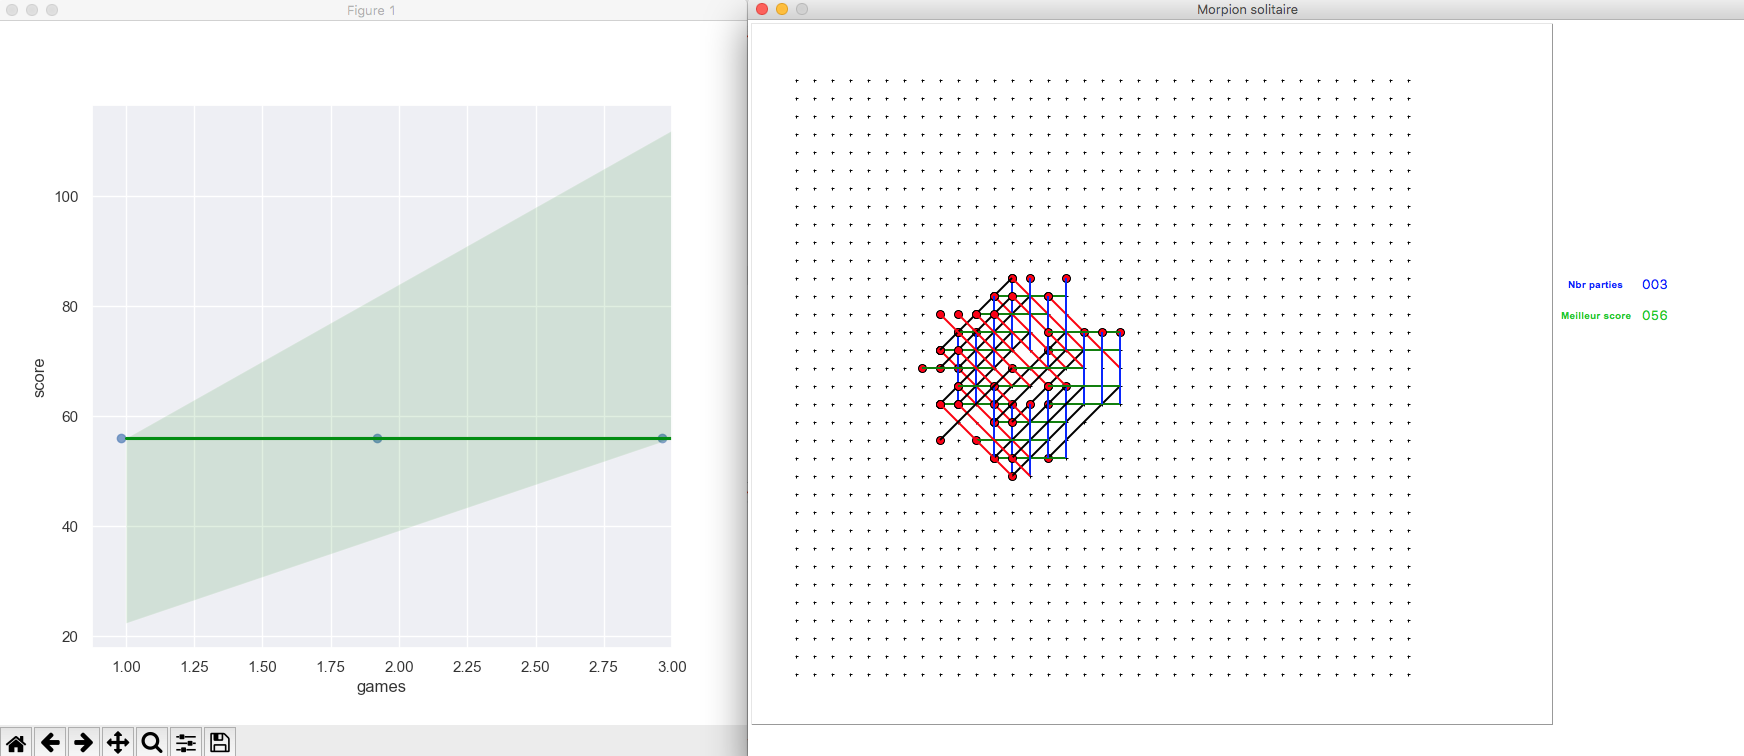
\includegraphics[scale=0.22]{ihm.png}
\\% 
\caption{The graphical interface - Example with 3 games played}
\end{figure}

\newpage
\subsection{Network connection}
\paragraph{}
\setlength{\parindent}{2cm}
The artificial neural network called 'agent' is contained in the 'DQN Py' file. This program is based for a long time on the Snake program with which we started this project. The network is composed of 3 layers, with 70 inputs and 8 outputs.

\begin{figure}[!h]
\centering
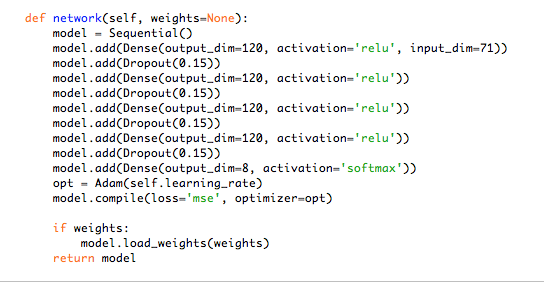
\includegraphics[scale=0.45]{state.png}
\\% 
\caption{Network Layer Creation Code}
\end{figure}
\paragraph{}
\setlength{\parindent}{2cm}
On a ajouté au programme un joueur, qui représente un point qui se déplace d'une distance d'un dans huit directions différentes dans le but de trouver une cellule qui représente le début d'une ligne jouable. Le joueur ou le point de déplacement est doté avec des coordonnées x et y (x-player, y-player).
\paragraph{}
\setlength{\parindent}{2cm}
The degree of freedom of the player is indicated in the range class and this indicates the maximum number of moves he is allowed to make according to a given output, to find a playable line otherwise he will crash. The agent contains an epsilon attribute that also indicates his freedom and this gives him the possibility, up to game 120 (chosen according to the best scores) to make random moves, so he can discover paths that could not have been explored with just a prediction and his game is deterministic. 
\begin{figure}[!h]
\centering
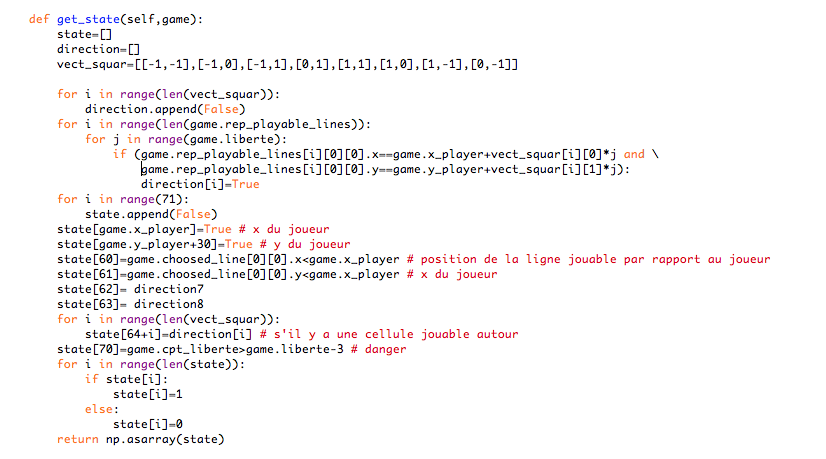
\includegraphics[scale=0.45]{couches.png}
\\% 
\caption{Coding of states}
\end{figure}

\paragraph{}
\setlength{\parindent}{2cm}
The game states are chosen to give the agent as much information as possible. There are 74 states, in the first 60 are used to indicate the position of the player.
\paragraph{}
\setlength{\parindent}{2cm}
Exemple: (x-player,y-player)=(3,4) This is equivalent in the states to
\newline
[0,0,0,1,0,0,0,0,0,0,0,0,0,0,0,0,0,0,0,0,0,0,0,0,0,0,0,0,
0,0,0,0,0,1,0,0,0,0,0,0,0,
\newline
0,0,0,0,0,0,0,0,0,0,0,0,0,0,0,0,0,0,0,0]
\paragraph{}
\setlength{\parindent}{2cm}
The logic was as follows, the first 30 bits indicate the x of the player (x-player) and from the 29th bit to 59th, it indicates the y position of the player (y-player).
\paragraph{}
\setlength{\parindent}{2cm}
Bits from 60 to 63 allow data an indication of the position of a randomly chosen playable cell at each game, in relation to the player.
\paragraph{}
\setlength{\parindent}{2cm}
The bits from the 64th to the 69th indicate, in relation to the player's position, whether there is a playable line the eight directions aligned.
\paragraph{}
\setlength{\parindent}{2cm}
The last input bit is used to indicate a crash hazard. It is set to one when the player has not found a playable line and has two moves left (2 clear distances) before crashing.
\paragraph{}
\setlength{\parindent}{2cm}
According to the steps of the game we will have a prediction that is an eight-bit output, in one, equal to one. This will indicate the direction for the player.
\paragraph{}
\setlength{\parindent}{2cm}
Exemple: An exit from the network = [1,0,0,0,0,0,0,0]
\paragraph{}
\setlength{\parindent}{2cm}
This is equivalent to applying the vector [-1, -1] to the player's coordinates (x-player, y-player), which means going diagonally right backwards with a distance of 1.

\paragraph{}
\setlength{\parindent}{2cm}
 The player loses, if he makes more than ten moves is found a playable line. At each crash, we check if the score reached is the best since the beginning of the game, we save the played lines in a list that we will use at the end for the display. 

\part{Achievements}
\section{Review of Achievements}
\subsection{Random mode}
\subsubsection{Functional Specification}
\paragraph{}
\setlength{\parindent}{2cm}
By using the "random" function that Python offers for random number generation, we produce a number that will be the index of a line in the list of playable lines. This sometimes, with tests between 10 games and 100 games can lead us into error by sometimes noticing improvements as games follow one another. The opposite has been demonstrated by doing tests with large numbers of games (figure 3 and 4). This shows us a constant line that is adequate with the random mode.
\subsubsection{Testes}
\begin{figure}[!h]
\centering
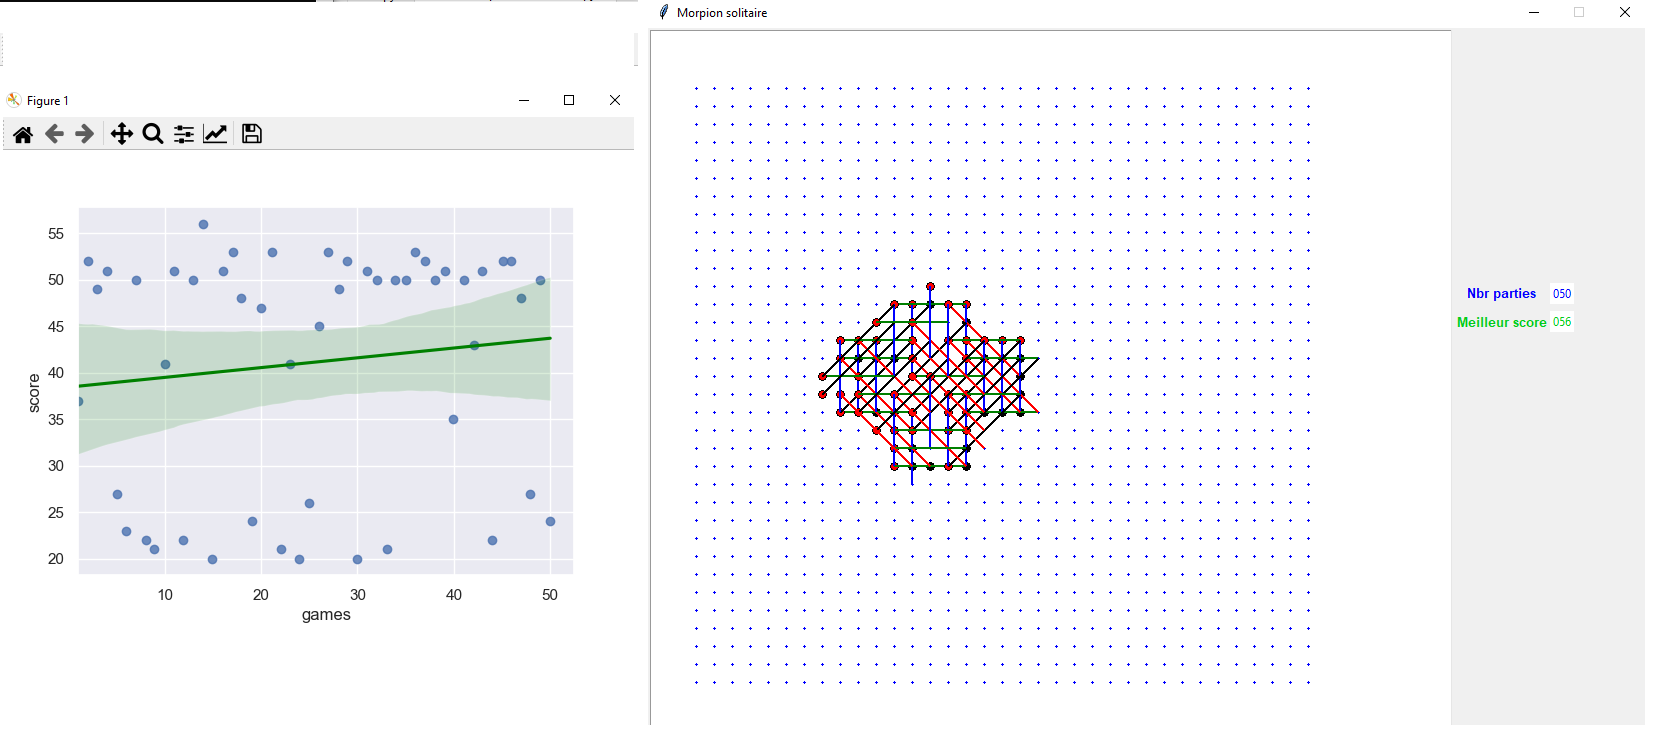
\includegraphics[scale=0.16]{test11.png}
\\% 
\caption{Random test result - 50 games}
\end{figure}

\begin{figure}[!h]
\centering
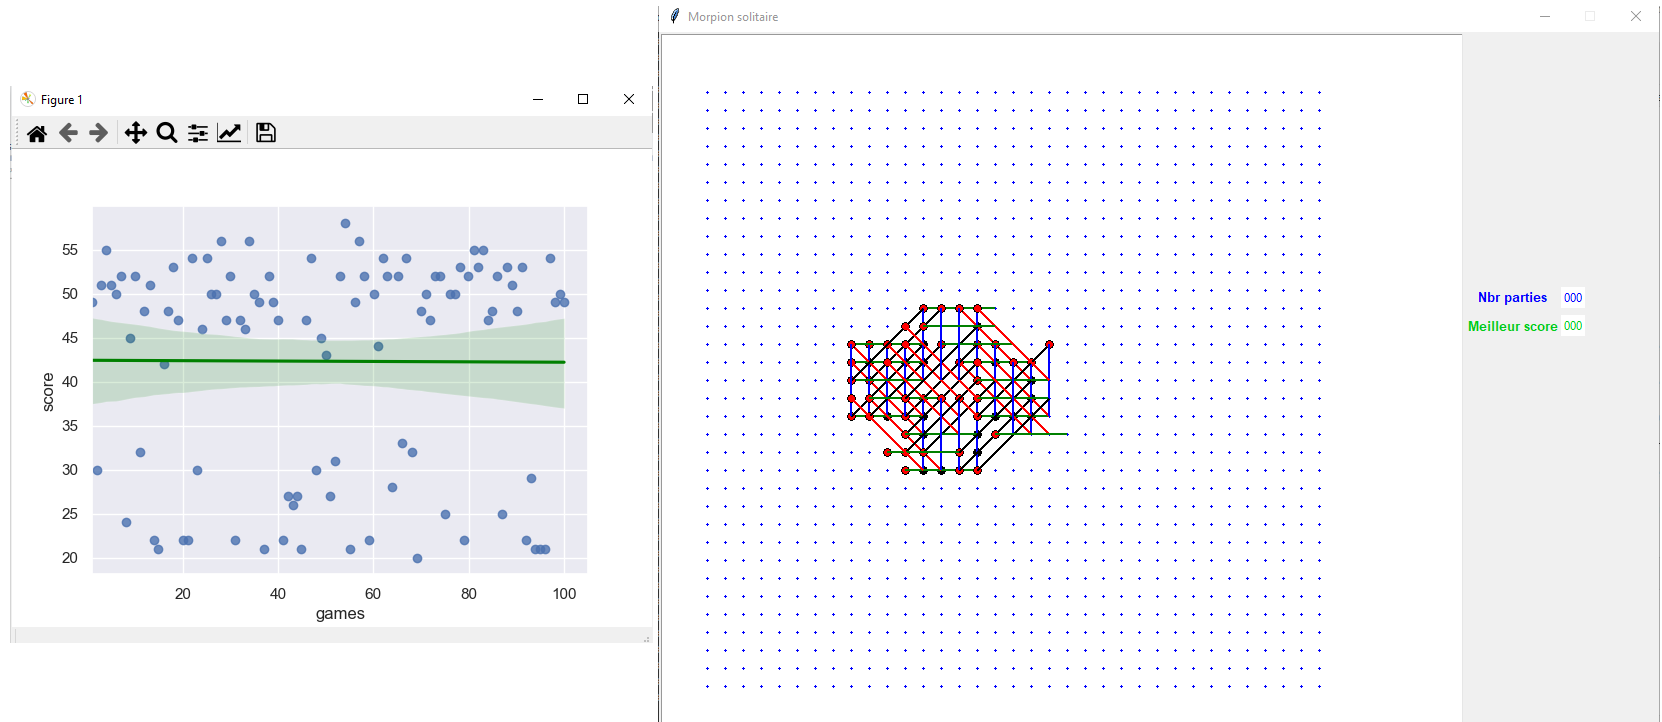
\includegraphics[scale=0.16]{test_aleatoire.png}
\\% 
\caption{Random test result - 100 games}
\end{figure}

\begin{figure}[!h]
\centering
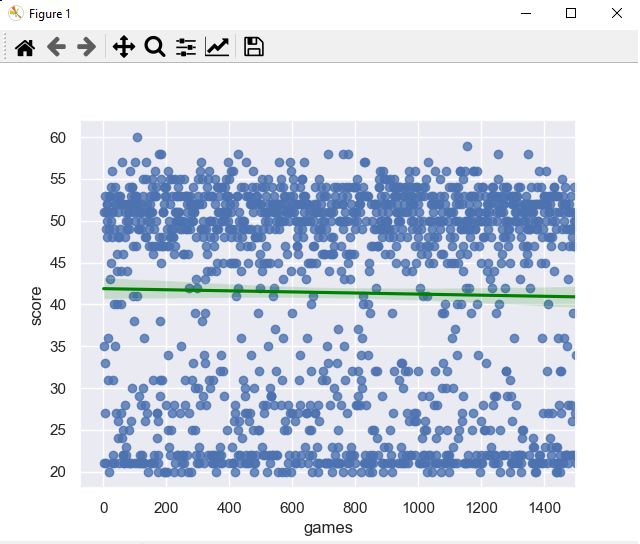
\includegraphics[scale=0.4]{test1000.png}
\\%
\caption{Random test result - 1000 games}
\end{figure}

\begin{figure}[!h]
\centering
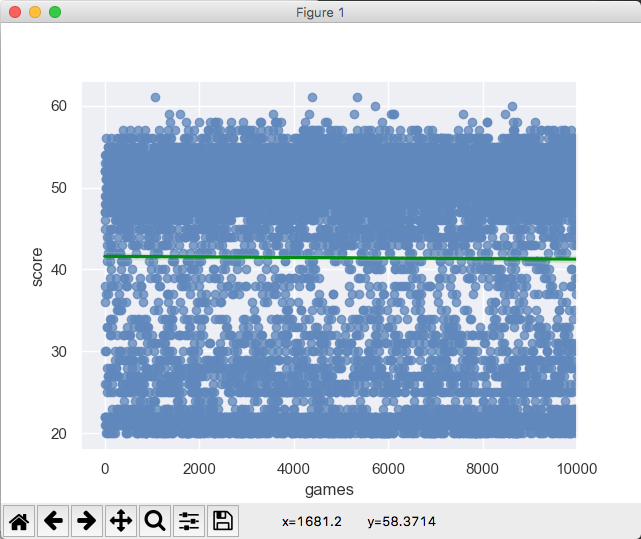
\includegraphics[scale=0.4]{1000.png}
\\% 
\caption{Random test result - 10 000 games}
\end{figure}

\subsection{Learning mode}
\subsubsection{Functional Specification}
\paragraph{}
\setlength{\parindent}{2cm}
In figures 8 and 9, we can see the progression of the game. In the first games, the player starts by discovering the field and thanks to the indications and his experience, he how to distinguish in which areas he accumulates the most reward. The best score reached after 400 games was 48 lines. In notice that the learning is done but it does not reach higher scores than the random mode. 
\subsubsection{Tests}
\begin{figure}[!h]
\centering
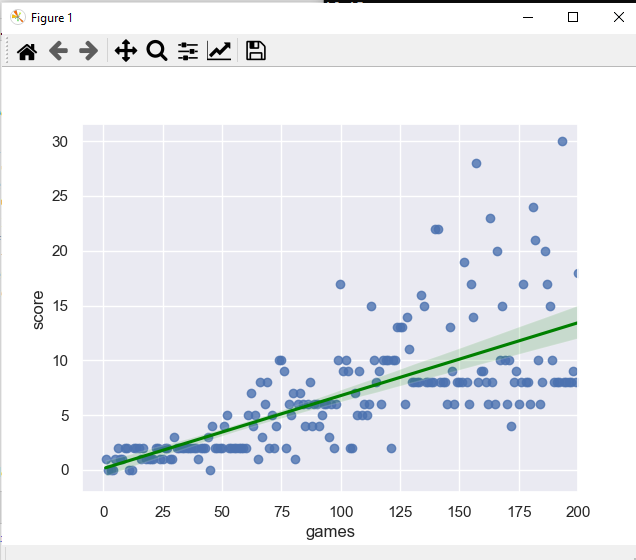
\includegraphics[scale=0.29]{tes2.png}
\\%
\caption{Result Q-Learning test - 200 games}
\end{figure}
\begin{figure}[!h]
\centering
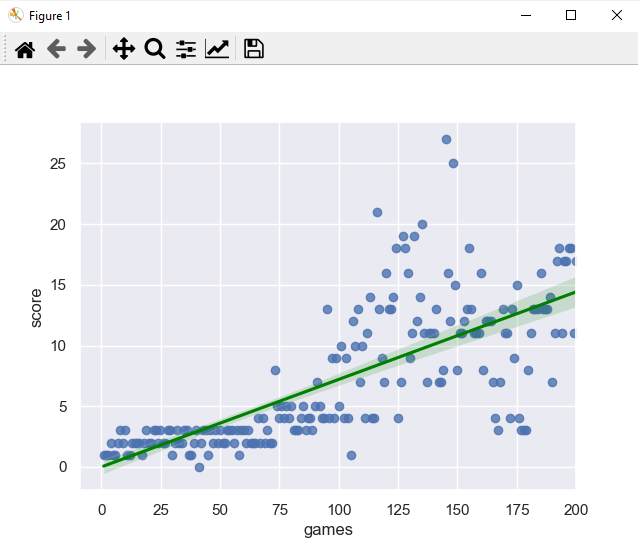
\includegraphics[scale=0.29]{test3.png}
\\%
\caption{Result Q-Learning test - 200 games}
\end{figure}
\subsection{Best random mode and learning parts}
\begin{figure}[!h]
\centering
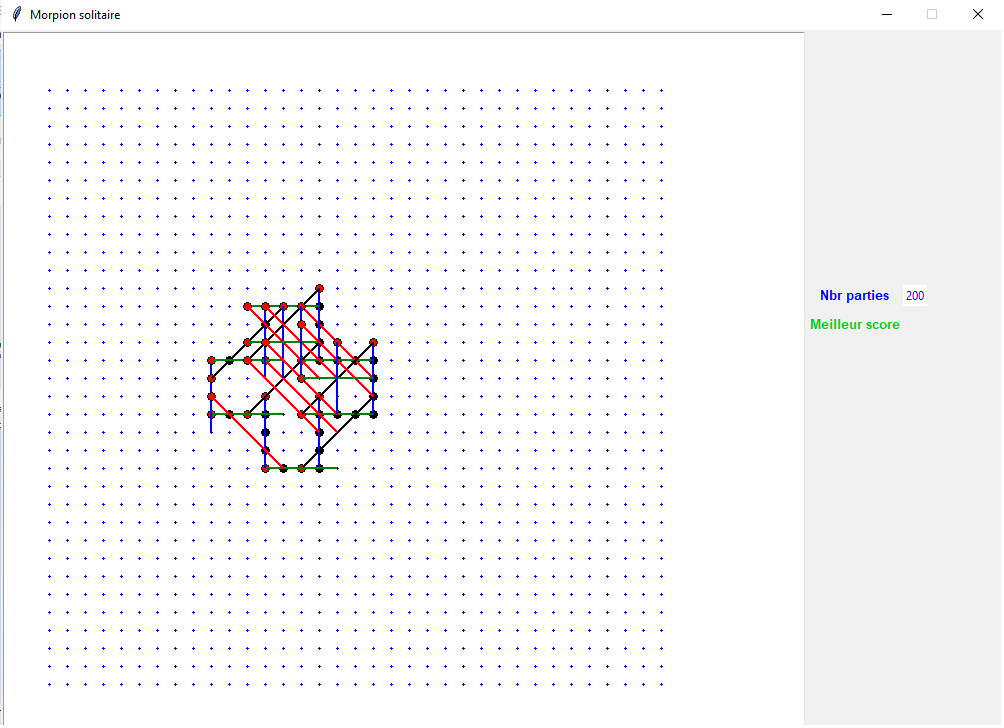
\includegraphics[scale=0.3]{test33.png}
\\%
\caption{One of the best games in Q-Learning mode - 200 games}
\end{figure}
\begin{figure}[!h]
\centering
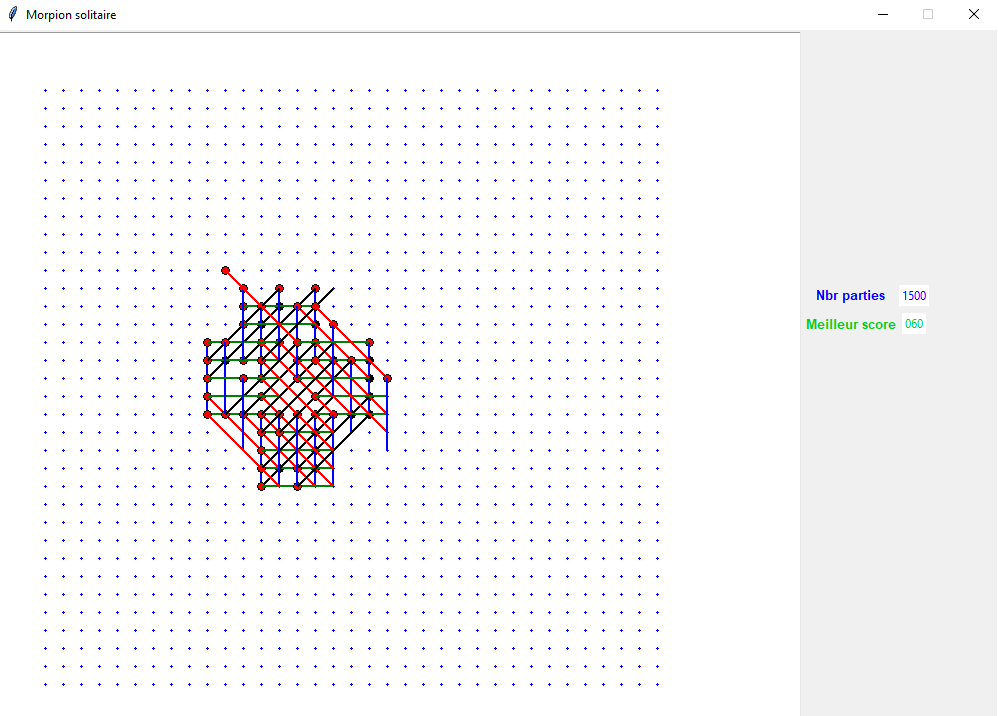
\includegraphics[scale=0.305]{best.png}
\\%
\caption{Best game in random mode - 1000 parties}
\end{figure}
\newpage
\section{Conclusion}
\paragraph{}
\setlength{\parindent}{2cm}
As part of our synthesis project, we designed and developed an algorithm for the Solitaire Morpion reinforcement learning game in order to optimize its score. Our solution offers a clean code and an ergonomic, simple and coherent interface while ensuring ease of use for a preliminary research team wishing to push the research for a better score. This report covers the study, design and implementation of the solution.
\paragraph{}
\setlength{\parindent}{2cm}
First, we began by studying the general context of the game. Then, we prepared a work schedule respecting the priorities of our needs. However, we started studying a solution for the game Snake, which could be similar to ours.
\paragraph{}
\setlength{\parindent}{2cm}
Throughout this period, we spent more time optimizing the code and learning how an artificial neural network works. Indeed, we encountered difficulties in configuring the Tensorflow environment, finding free slots to meet with our tutor and the current health crisis which did not help the situation either. In addition, we spent a lot of time coding the algorithm. The contribution of this work has been very important because it has allowed us: to follow a well-studied working method, to deepen my knowledge in the field of artificial intelligence and to master the shortcuts offered by the Python language. On the technical aspect, this project was approached to ? n ensure an optimized algorithm of the game and this thanks to various exchanges with our tutor Denis ROBILLIARD who gave us the benefit of his experience despite the problems encountered during this crisis. Indeed, taking charge of such a project in this framework certainly allows us to develop our spirit of analysis, reflection and decision.
\paragraph{}
\setlength{\parindent}{2cm}
In the end, our work is not finished there. We aim at optimizing the neural network with new tests that will determine the number of layers to which the algorithm is sensitive. Finally, we can extend the algorithm by adding new optimizations that we did not consider in the first study. For example, we can add another artificial intelligence that will take into account the best games reached in this game.
\newpage
\bibliographystyle{plain}
\bibliography{references}
\end{document}